\section{Tasks and Requirements}
\subsection{DeSCENT}

On the DeSCENT mission there is still a lot of work to be done over the year. There is significant amounts of work to be done on the power and RF side of the V1 chipsat We are just beginning the work of a new version of the DeSCENT chipsat 
%%%%%%%%%%%%%%%%%%%
durrently dubbed v2 - but hopefully changing to Tiberius.
%%%%%%%%%%%%%%%%%%%
On this new version some of the major work to be done is:
\begin{enumerate}
    \item WIO-E5 footprinting
    \item WIO-E5 PCB implementation
    \item Breadboarding to test WIO-E5 circuitry
    \item Testing of PCBs when they arrive
    \item Power testing and design \begin{enumerate}
        \item Falling weight balance
        \item Maple seed design
            \end{enumerate}
    \item Breadboarding and testing of both v1 and v2
\end{enumerate}
\begin{figure}[H]
    \begin{center}
            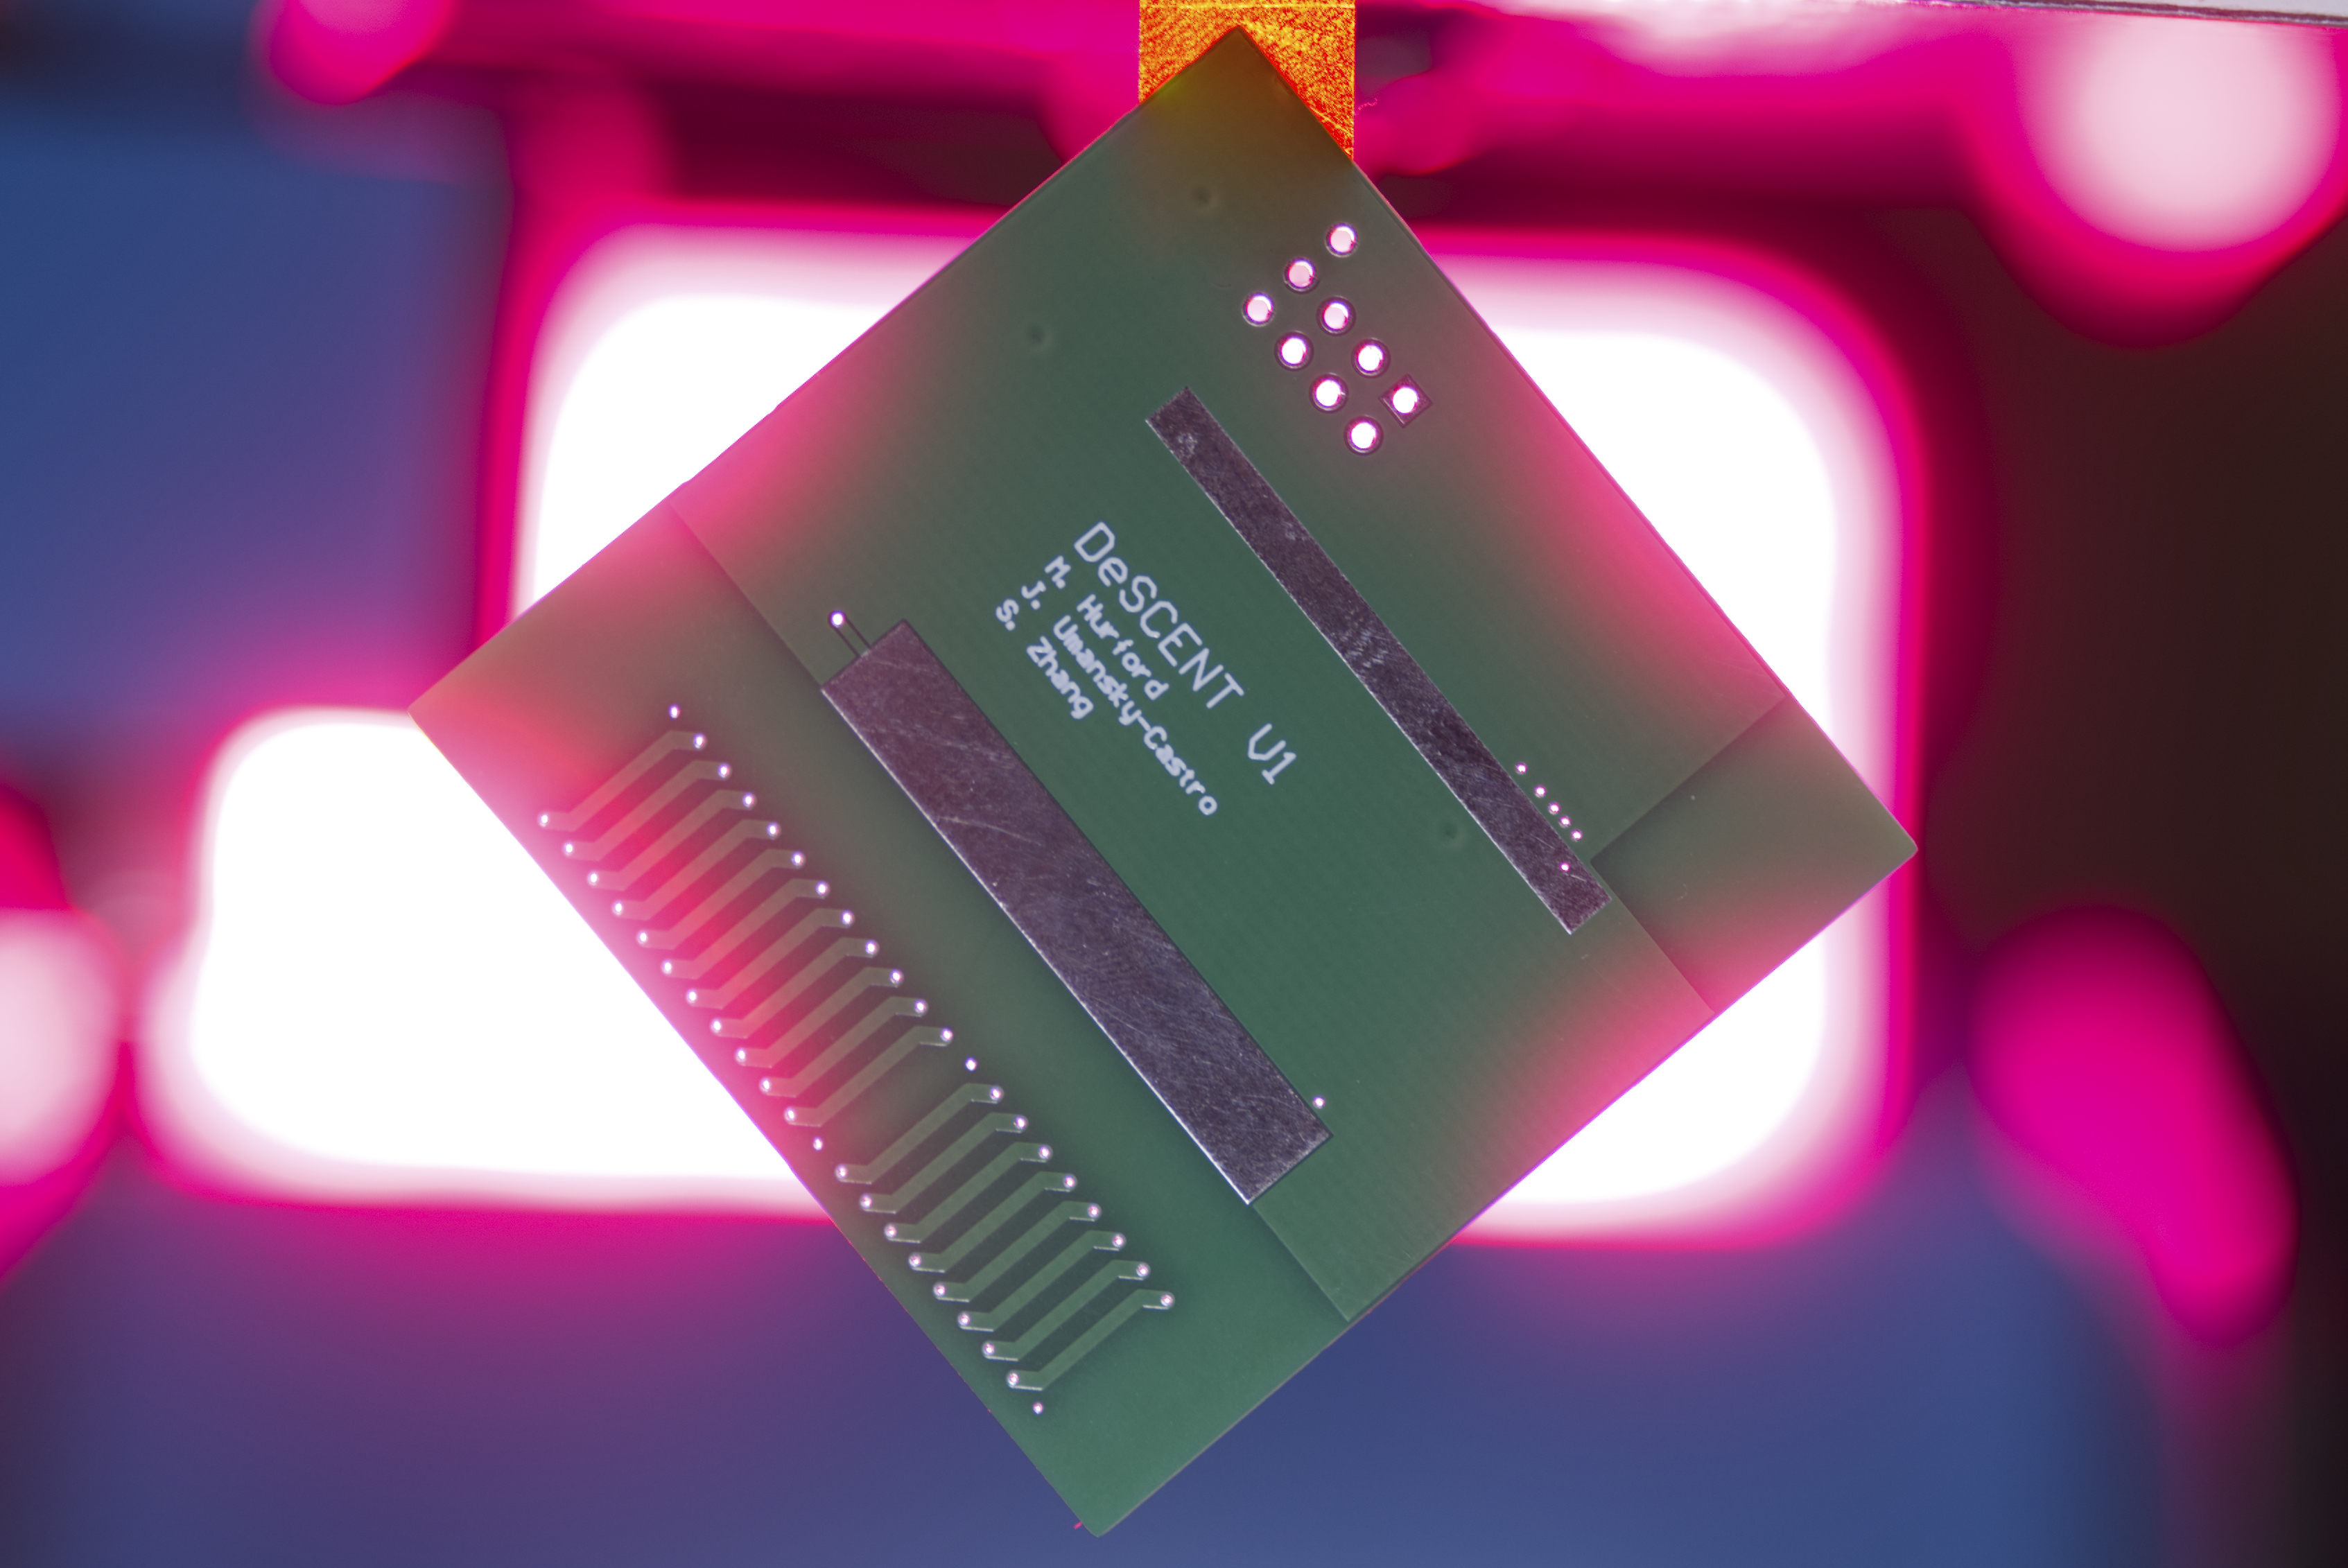
\includegraphics[width=.9\textwidth]{Images/Descent.jpg}\caption{Version one of the DeSCENT ChipSat.}
    \end{center}
\end{figure}

\subsection{Alpha ChipSat and Picoballoon}

As far as the Alpha ChipSat goes there is far less to do. Mainly involving finishing touches and testing the infrastructe that we are planning to use for communications once in space. The infrastructure test will be done using a high altitude balloon. Some goals for this part of the project are:
\begin{enumerate}
    \item Validate balloon test solar setup \begin{enumerate}
        \item Power is on and consistant throughout flight
        \item Longer duration than the last flight -- both signals dropped at 90ß minutes.
        \item Able to transmit consistently -- very power hungry
    \end{enumerate}
    \item Launch balloon test
    \item circumnavigate the globe with the high altitude balloon
    \item Solve GPS power up issue
\end{enumerate}
\begin{figure}[H]
    \begin{center}
            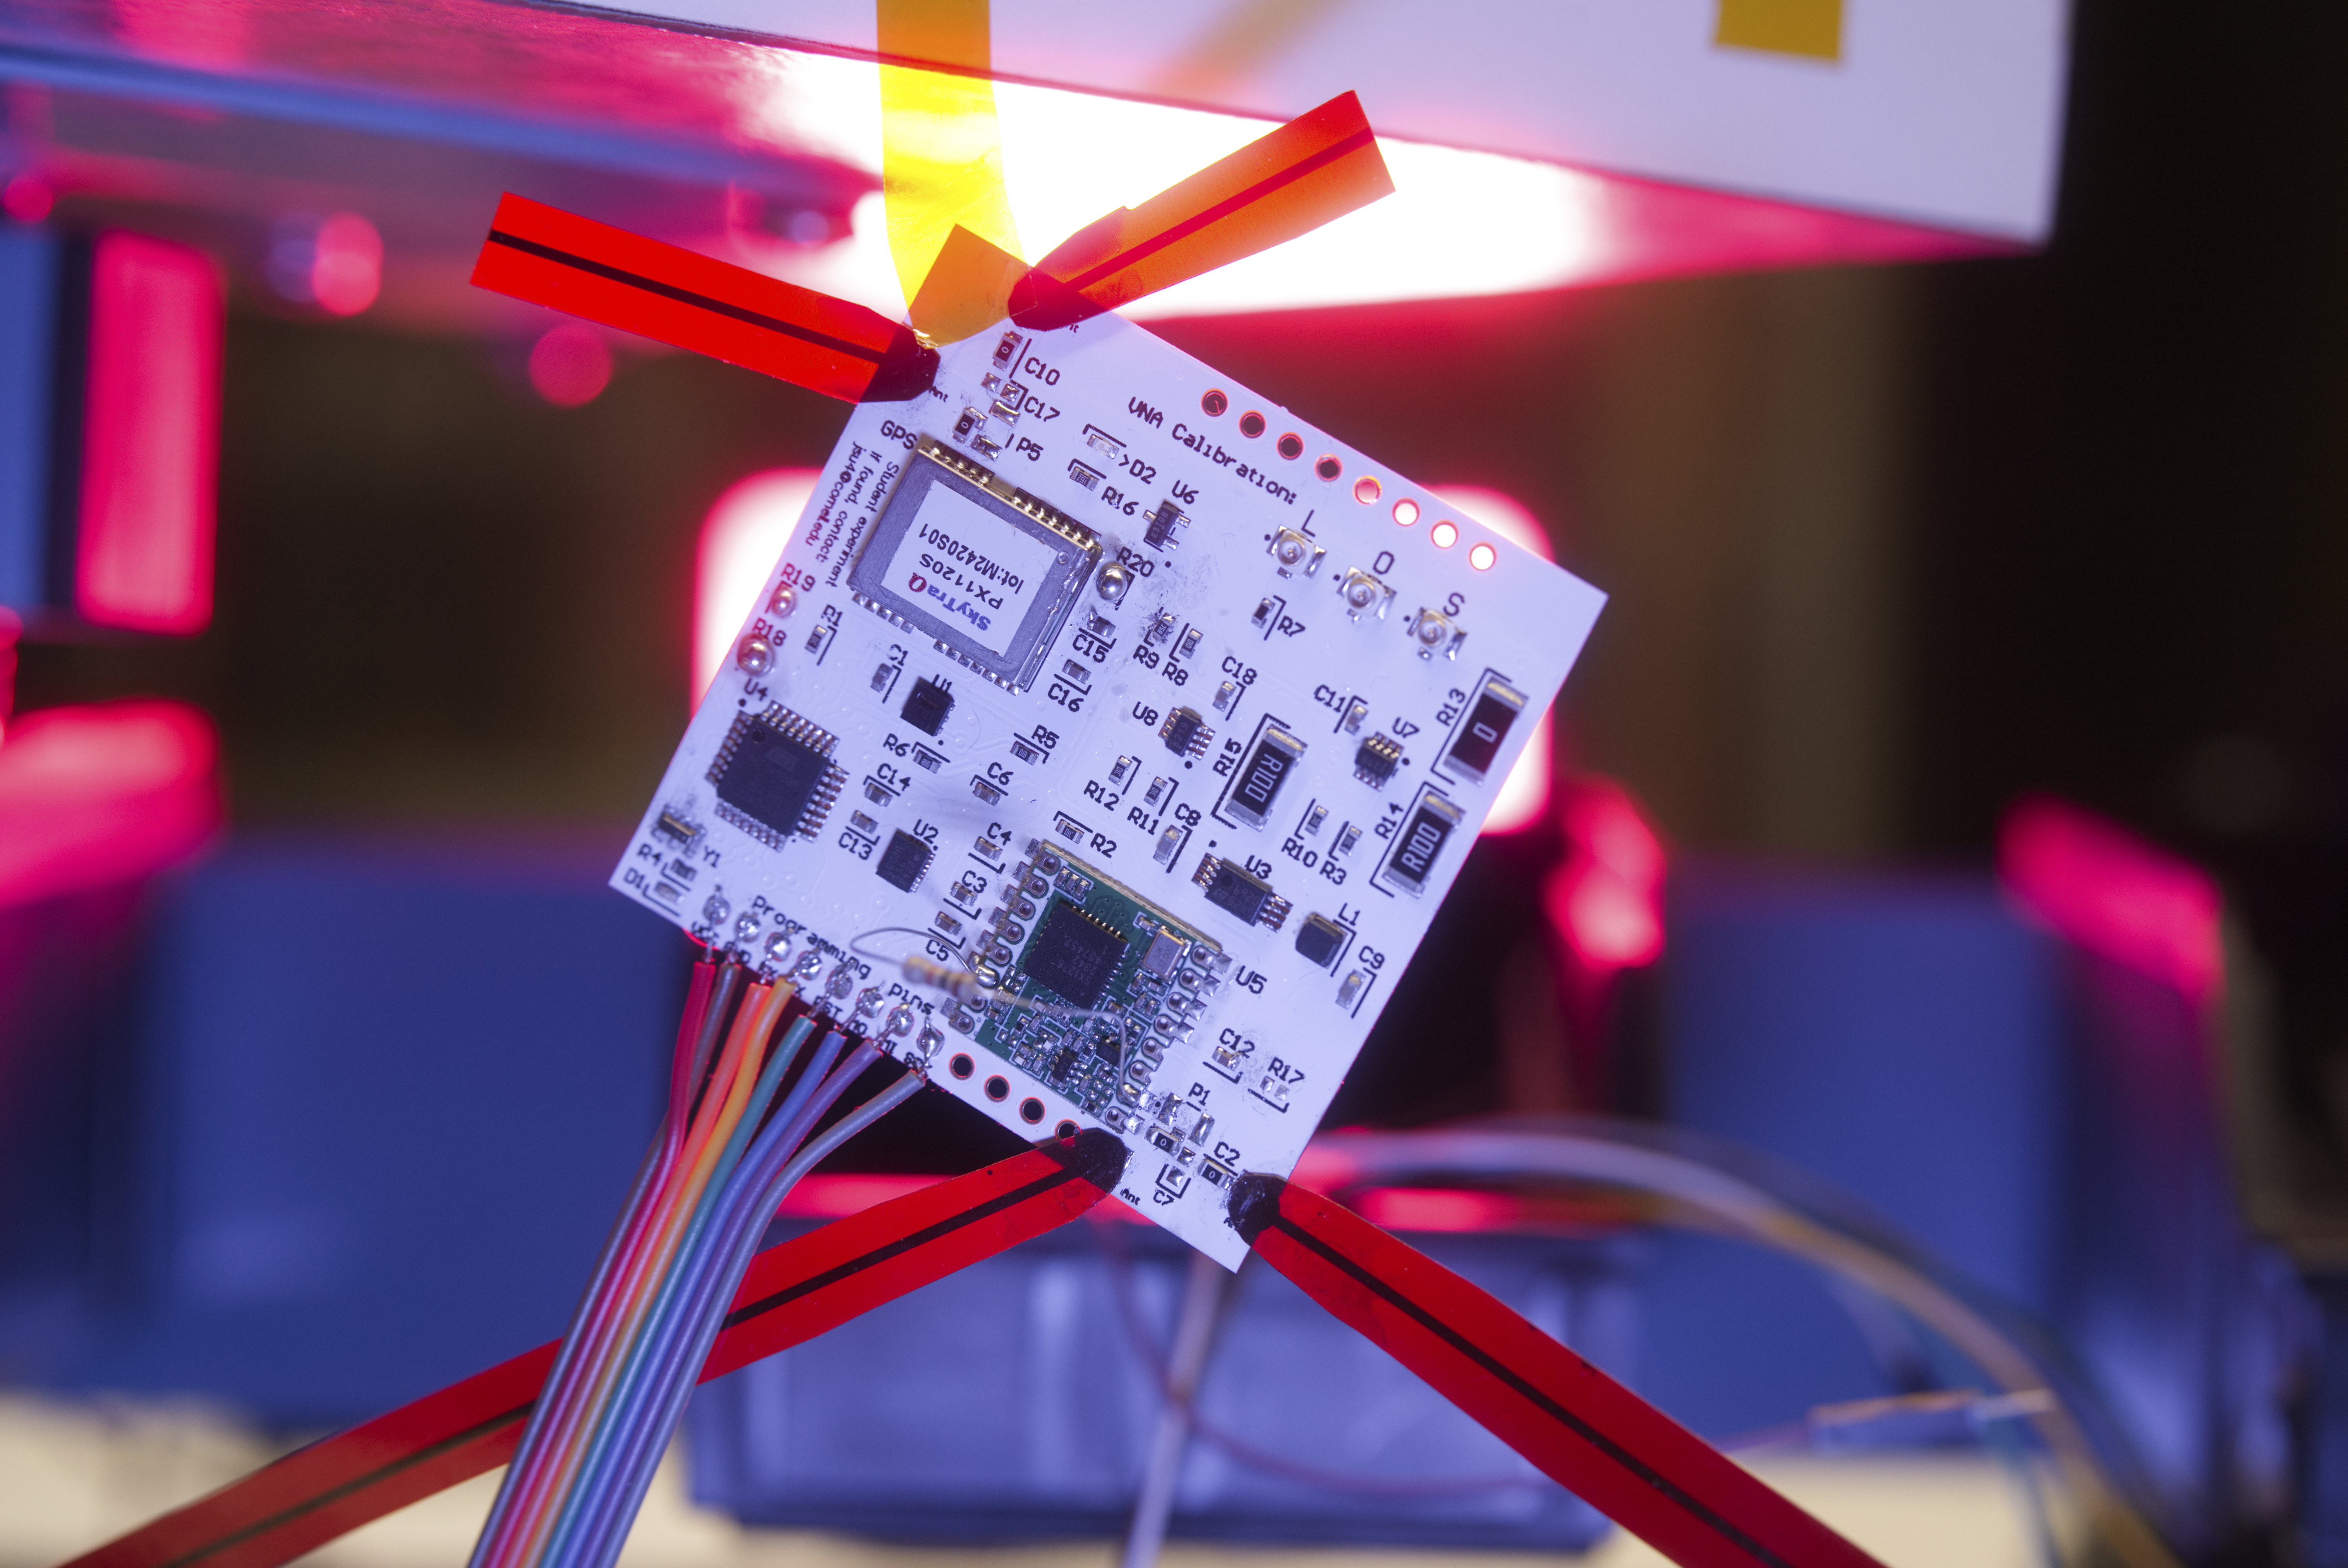
\includegraphics[width=.9\textwidth]{Images/Alpha.jpg}\caption{A current Alpha ChipSat.}
    \end{center}
\end{figure}